\documentclass[usenames,dvipsnames]{beamer}
\usepackage[utf8]{inputenc}
\usepackage[T1]{fontenc}
\usepackage[francais]{babel}
\usepackage{xcolor}
\usepackage{packages/tikz-uml}
\usetheme{Singapore} %Boadilla | Bergen | Madrid | Antibes | Hannover | Singapore | Warsaw
%----------------------------------------------------------------------------------------
%   TITLE INFORMATION
%----------------------------------------------------------------------------------------
\title{LaRuche}
\subtitle{HLSE602 -- Projet CMI Annuel}
\author{B. Rima \and O. Farajallah \and W. Soussi}
\institute[UM]{L3 CMI Informatique}
\date{\today}

\begin{document}
%----------------------------------------------------------------------------------------
%   TITLE FRAME
%----------------------------------------------------------------------------------------
\begin{frame}
\titlepage
\end{frame}
%----------------------------------------------------------------------------------------
%   OUTLINE
%----------------------------------------------------------------------------------------
\begin{frame}{Sommaire}
\tableofcontents
\end{frame}
%----------------------------------------------------------------------------------------
%   INTRODUCTION
%----------------------------------------------------------------------------------------
\section{Introduction}
\begin{frame}{Contexte du projet}{Introduction}
  \begin{description}
    \item [Projet CMI :] Module d'un projet annuel pour l'année 2017--2018 dans le cadre du \textbf{CMI Informatique}.
    \item [Responsable CMI Informatique :] Mme Anne-Elisabeth Baert.
    \item [Encadrant du projet :] M. Eric Bourreau.
    \item [Lieux de travail :] La \textbf{FDS} et le \textbf{LIRMM}.
  \end{description}
\end{frame}

%----------------------------------------------------------------------------------------
%   PROBLÉMATIQUE ET MÉTHODOLOGIE DE RÉSOLUTION
%----------------------------------------------------------------------------------------
\section{Problématique et Méthodologie de Résolution}
\subsection{Problématique}
\begin{frame}{Problématique}{Problématique et Méthodologie de Résolution}
\begin{columns}[onlytextwidth, T]
  \column{55mm}
    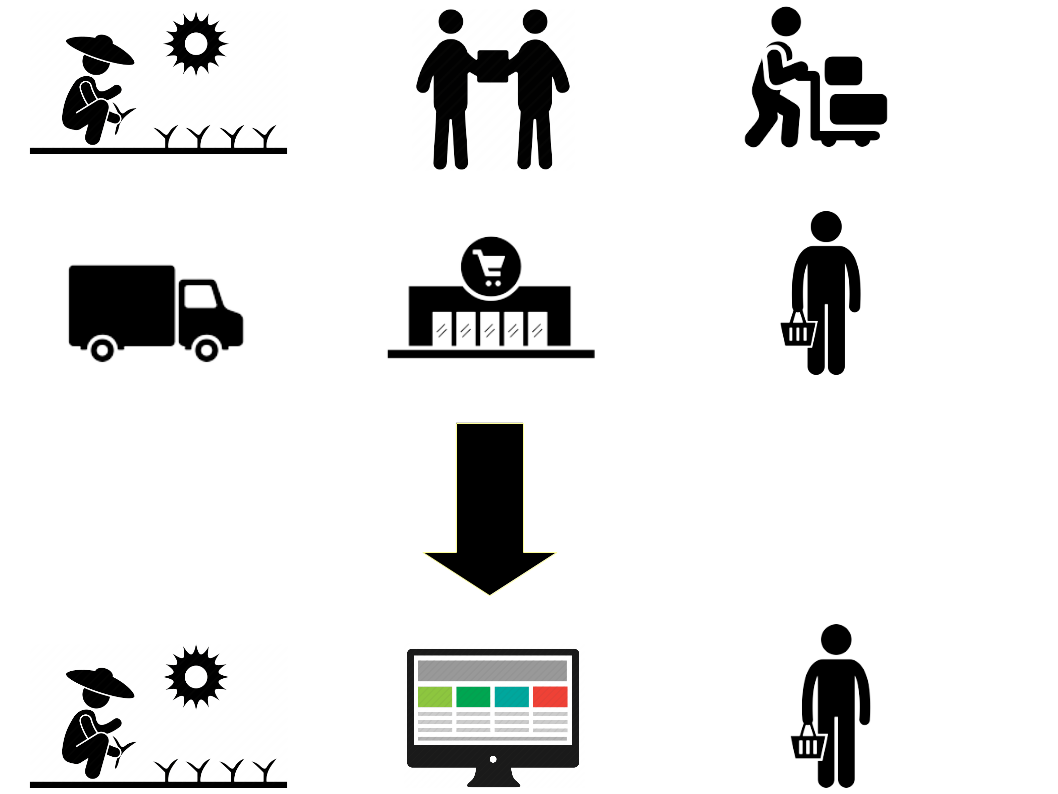
\includegraphics[scale=0.2]{images/chain_production.png}

  \column{\dimexpr\linewidth-40mm-2mm}
    \begin{block}{Consommateurs :}
    Acheter des produits frais et minimiser les étapes de processing.
    \end{block}

    \begin{block}{Producteurs :}
      Maîtriser le prix de vente et les débouchés de leurs productions en se libérant des intermédiaires de distribution.
    \end{block}
\end{columns}
\end{frame}

\subsection{Solutions}
\begin{frame}{Solution possible : La Ruche Qui Dit Oui}{Problématique et Méthodologie de Résolution}
\begin{block}{Site Web}
Une interface directe entre \textbf{consommateurs} et \textbf{fournisseurs}.
\end{block}

\begin{definition}[Ruche]
Un regroupement de plusieurs membres \textbf{consommateurs} et \textbf{fournisseurs} d'une région, guidé par un \textbf{responsable de ruche}.
\end{definition}

\begin{block}{Vision Centralisée}
\begin{itemize}
  \item l'ensemble des ruches obeit à une entité centrale : la \textbf{Ruche-Mama}.
  \item la \textbf{Ruche-Mama} s'occupe de la gestion des ruches : création, réglementations internes, interactions, évolution et extensibilité des services, $\dots$.
\end{itemize}
\end{block}
\end{frame}

\begin{frame}{Solution proposée : \texttt{LaRuche}}{Problématique et Méthodologie de Résolution}
\begin{block}{Site Web}
Une interface directe entre \textbf{consommateurs} et \textbf{fournisseurs}.
\end{block}

\begin{definition}[Ruche]
Un regroupement de plusieurs \textbf{fournisseurs} d'une région, \textbf{sans guide explicite} préfixé par le site.
\end{definition}

\begin{block}{Vision Décentralisée et Autonome}
\begin{itemize}
  \item l'ensemble des ruches ne répond à \textbf{aucune entité centrale}.
  \item chaque ruche s'occupe de ses propres besoins et de leur gestion sans besoin d'un intermédiaire et d'une hiérarchie à respecter.
\end{itemize}
\end{block}
\end{frame}

\subsection{Méthodes agiles}
\begin{frame}{Méthodologie de résolution : méthodes agiles}{Problématique et Méthodologie de Résolution}
\begin{block}{Méthodes Agiles}
Une approche de développement logiciel de plus en plus prépondérante basée sur une conception/développement itérative, orientée-test et orientée-client.
\end{block}

\begin{block}{Pourquoi ?}
\begin{itemize}
  \item meilleure gestion des ressources
  \item sortie plus fréquente de versions fonctionnelles et testées du produit
  \item interaction plus fréquente avec les clients : adaptation et extensibilité du produit selon leurs besoins
\end{itemize}
\end{block}
\end{frame}
%----------------------------------------------------------------------------------------
%   CONCEPTION
%----------------------------------------------------------------------------------------
\section{Conception}
\subsection{Outils de conception utilisés}

\begin{frame}{Outils de conception utilisés}{Conception}
\begin{enumerate}
  \item Diagrammes de cas d'usage
  \item Modèle EA
  \item Schéma de base de données
  \item \textit{Storyboard}
\end{enumerate}
\end{frame}

% \subsection{\protect\textit{User Stories} : outil de conception agile}
\begin{frame}{\textit{User Stories} : outil de conception agile}{Conception}
\begin{block}{\textit{User Stories}}
Des requis fournis par les clients, décrivant en langage naturel les fonctionnalités qu'ils souhaitent avoir dans le produit développé.
\end{block}

\begin{block}{\textcolor{Sepia}{\texttt{Intitulé}}}
\begin{it}
  En tant que \textcolor{DarkOrchid}{\texttt{<rôle>}}, je souhaite \textcolor{BrickRed}{\texttt{<fonctionnalité>}}, \\
  ~~~~~~~~~dans le but de \textcolor{OliveGreen}{\texttt{<bénéfice>}}.
\end{it}
\end{block}
\end{frame}

\subsection{Besoins}
\begin{frame}{Besoins}{Conception}
\begin{block}{Besoins}
\begin{enumerate}
  \item Des profils d'utilisateurs \textbf{fournisseur/client} : propriétés et fonctionnalités via des \textit{user-stories}.
  \item Une \textbf{structure de données} pour décrire le \textbf{regroupement des fournisseurs} et leurs \textbf{interactions} : \texttt{ruche}, \texttt{opérateur cellule}, \texttt{voisins}, $\dots$
\end{enumerate}
\end{block}
\end{frame}

\subsection{Côté fournisseur}
\subsubsection*{Ruche : Structure de données proposée}
\begin{frame}{Côté fournisseur}{Ruche : Structure de données proposée}
\begin{block}{Définitions de base}
\begin{description}
  \item[$\textbf{V}$]{ensemble des fournisseurs.}
  \item[$\textbf{C}$]{ensemble des clients.}
  \item[$\pi_v$]{\textbf{opérateur} appliqué à $v \in V$, désignant une \textbf{cellule}, c.à.d. un \textbf{cercle} dont le centre est le point représentant les coordonnées du fournisseur $v$ et dont le rayon est la distance maximale en \textbf{km} qu'il souhaite parcourir afin de se rendre à un lieu de collecte.}
\end{description}
\end{block}
\end{frame}

\begin{frame}{Côté fournisseur}{Ruche : Structure de données proposée($2$)}
\begin{block}{Ruche}
Soit $v_1, v_2, \dots, v_n \in V^n$. Une \textbf{ruche} $R = (p, V_R)$ est composée de :
\begin{description}
  \item[$\mathbf{V_R}$]{ensemble de fournisseurs dont les cellules s'intersectent;}
  \item[$\mathbf{p}$]{un point de collecte obtenu à partir d'une opération\footnote{le choix du point est relatif aux fournisseurs de la ruche, étant indéterministe en soi} sur la zone d'intersection des cellules correspondantes aux vendeurs de $V$.}
\end{description}
Autrement dit, $R = \{p, \{v_1, v_2, \dots, v_n \in V\; |\; \pi_{v_1} \cap \pi_{v_2} \cap \dots \cap \pi_{v_2} \neq \varnothing\}\}$
\end{block}
\end{frame}

\begin{frame}{Côté fournisseur}{Ruche : Structure de données proposée($3$)}
\begin{figure}[!ht]
  \centering
  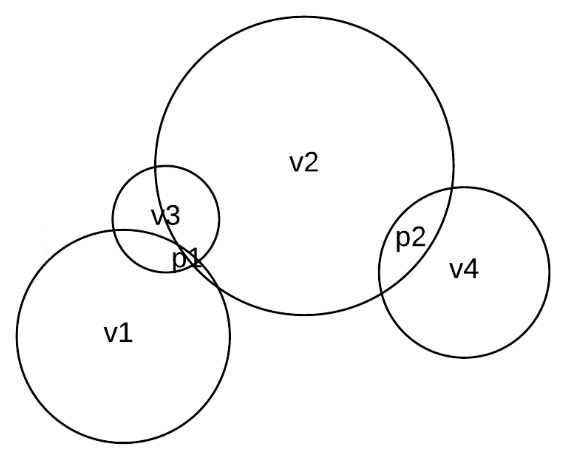
\includegraphics[scale=0.17]{images/exemple_introductif1.png}
\end{figure}

\begin{block}{Appartenance Simultanée}
Un fournisseur peut appartenir à plusieurs ruches simultanément.
\end{block}

\begin{block}{Fournisseurs Voisins}
Soit $R = \{p, V_R\}$ une ruche. Deux fournisseurs $v_1$ et $v_2$ sont dits \textbf{voisins} $\iff v_1 \in V_R\; \text{et}\; v_2 \in V_R$. On note $\texttt{Voisins}(v)$ l'\textbf{ensemble des voisins} d'un fournisseur $v$, contenant \textbf{tous les voisins} de \textbf{toutes les ruches} auxquelles il appartient.
\end{block}
\end{frame}

\begin{frame}{Côté fournisseur}{Ruche : Structure de données proposée($4$)}
\begin{figure}[!ht]
  \centering
  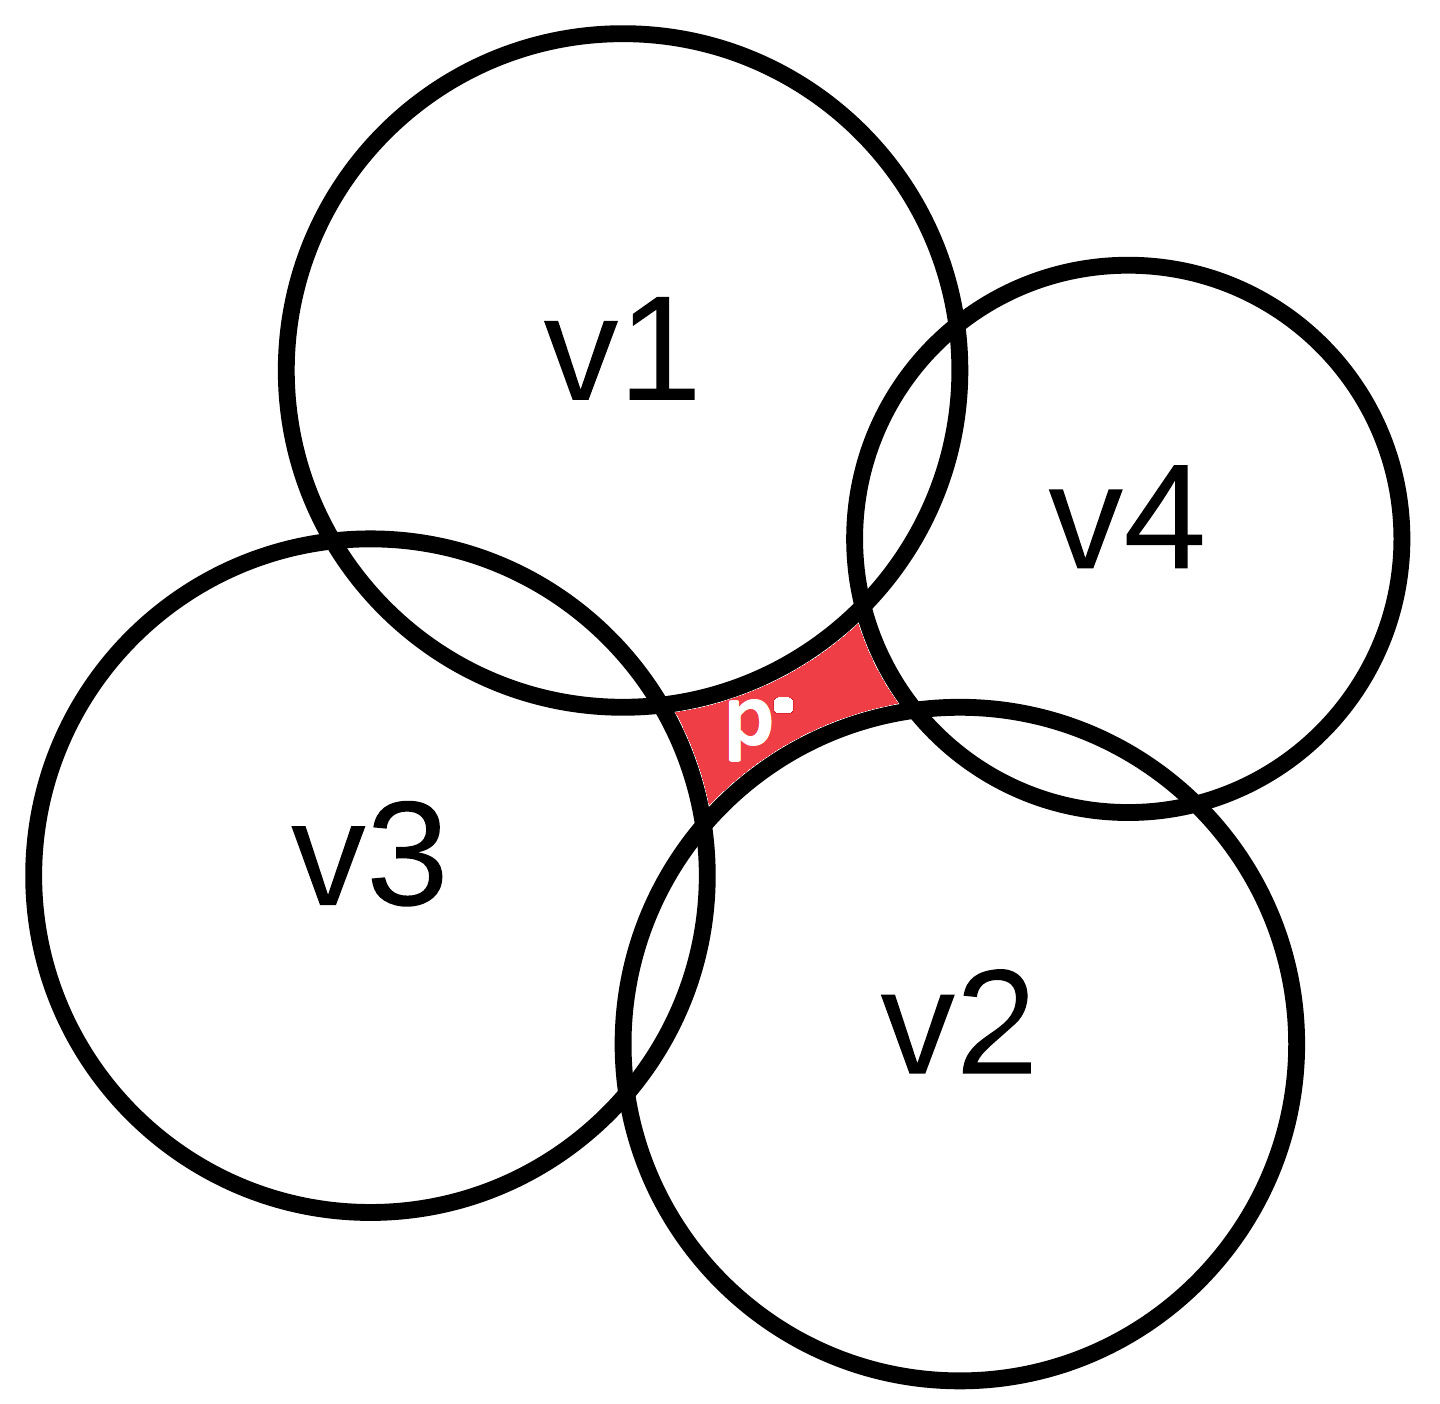
\includegraphics[scale=0.08]{images/exemple_introductif2.png}
\end{figure}

\begin{block}{Voisinage Imposé}
Soient $v_1$ et $v_2$ deux fournisseurs tels que $v_2 \notin \texttt{Voisins}(v_1)$. S'il existe des fournisseurs $v_3$ et $v_4$ tels que $v_3, v_4 \in \texttt{Voisins}(v_1) \cap \texttt{Voisins}(v_2)$ et $v_3 \notin \texttt{Voisins}(v_4)$, alors il existe une ruche plus optimale contenant $v_1, v_2, v_3\; \text{et}\; v_4$ que les ruches séparées les contenant.
\end{block}
\end{frame}

\subsubsection*{\protect\textit{User-stories} des fournisseurs}
\begin{frame}{Côté fournisseur}{Intitulés des \textit{user-stories} fournisseur}
\begin{enumerate}
  \item Définition et stockage de produits.
  \item Offre de Paniers.
  \item Rapports de suivi périodiques.
  \item Politique de rupture des stocks.
  \item Politique de partage entre ruches.
  \item Validation de commandes.
  \item Attribution de factures.
\end{enumerate}
\end{frame}

\begin{frame}{Côté fournisseur}{Exemple d'une \textit{user-story} fournisseur}
\begin{block}{\textcolor{Sepia}{\texttt{Définition et stockage de produits}}}
En tant que \textcolor{DarkOrchid}{fournisseur}, je souhaite {\color{BrickRed} \textbf{définir} ma \textbf{sélection de produits} selon des \textbf{informations caractéristiques} à fournir dans des \textbf{formulaires}},\\
~~~~~~~~~dans le but de {\color{OliveGreen}maximiser la transparence de mes produits pour gagner la fidelité de mes clients, tout en \textbf{gérant} (création, modification, ajout, suppression) ma sélection à travers le site}.
\end{block}
\end{frame}

\subsubsection*{Profil fournisseur}
\begin{frame}{Côté fournisseur}{Profil fournisseur}
\begin{enumerate}
  \item Un fournisseur offre des produits/paniers divers.
  \item Un fournisseur gére ses produits/paniers dans des stocks.
  \item Un fournisseur suit l'évolution de ses ressources via des rapports de suivi périodiques.
  \item Un fournisseur interagit :
  \begin{itemize}
    \item avec d'autres \textbf{fournisseurs} pour créer des ruches et organiser des évènements de collecte.
    \item avec les \textbf{clients} qui l'ont déjà contacté.
  \end{itemize}
\end{enumerate}
\end{frame}

\begin{frame}{Côté fournisseur}{Profil fournisseur($2$)}
\begin{enumerate}
  \item Un fournisseur valide les commandes de réservation des produits.
  \item Un fournisseur règle les commandes physiquement, en premier temps, et puis via le site dans les versions ultérieures.
  \item Un fournisseur imprime les factures, créées par le site lors de la réservation des produits par des clients, et les émet aux clients correspondants lors de la collecte de leurs produits.
\end{enumerate}
\end{frame}

\begin{frame}{Côté fournisseur}{Page d'accueil de l'utilisateur fournisseur}
\begin{figure}[!ht]
  \centering
  \resizebox{0.75\textwidth}{!}{
    \begin{tikzpicture}
      \setcounter{tikzumlUseCaseNum}{0}
      \umlactor[x=-1, y=-1]{Vendor}
      \umlactor[x=8, y=-1]{Database}
      \begin{umlsystem}[x=3, fill=green!10]{home page}
        \umlusecase[width=3cm]{Add/Delete/Modify Products}
        \umlusecase[y=-2.5, width=3cm]{Add/Delete/Modify Baskets}
        \umlusecase[y=-4.5]{Check Stocks}
        \umlusecase[y=-6.5]{Check Reports}
      \end{umlsystem}
      \umlextend[name=ext]{usecase-2}{usecase-1}
      \umlextend{usecase-4}{usecase-3}
      \umlassoc{Vendor}{usecase-1}
      \umlassoc{Vendor}{usecase-2}
      \umlassoc{Vendor}{usecase-3}
      \umlassoc{Vendor}{usecase-4}
      \umlassoc{Database}{usecase-1}
      \umlassoc{Database}{usecase-2}
      \umlassoc{Database}{usecase-3}
      \umlassoc{Database}{usecase-4}
      \umlnote[x=-2, y=-4]{ext-1}{Products have to exist in the database prior to the introduction of baskets}
    \end{tikzpicture}
  }
\end{figure}
\end{frame}

\begin{frame}{Côté fournisseur}{Gestion des commandes du point de vue du fournisseur}
  \begin{figure}[!ht]
   \centering
   \resizebox{0.65\textwidth}{!}{
     \begin{tikzpicture}
       \setcounter{tikzumlUseCaseNum}{0}
       \umlactor{Vendor}
       \umlactor[x=12, y=-2]{Database}
       \umlactor[x=12, y=-5]{Client User Database}
       \umlactor[x=12, y=-7]{Bank/PayPal}
       \umlactor[x=12, y=-9]{Bill Reception Platform}
       \begin{umlsystem}[x=4, fill=red!10]{vendor home page}
         \umlusecase[width=2cm]{Check Stocks}
         \umlusecase[x=5, width=2cm]{Allow Delayed Orders}
         \umlusecase[x=2.6, y=-2, width=3cm]{Set Purchase Deadline}
         \umlusecase[x=4, y=-5, width=3cm]{Check Pending Orders}
         \umlusecase[y=-7, width=2cm]{Process Pending Orders}
         \umlusecase[x=5, y=-7, width=2cm]{Send Bill}
         \umlusecase[x=4.5, y=-10, width=2cm]{Update Sales' History}
       \end{umlsystem}
       \umlextend{usecase-2}{usecase-1}
       \umlextend[name=deadline]{usecase-3}{usecase-4}
       \umlextend[name=checkPending1]{usecase-4}{usecase-5}
       \umlinclude{usecase-5}{usecase-6}
       \umlinclude{usecase-6}{usecase-7}
       \umlassoc{Vendor}{usecase-1}
       \umlassoc[name=checkPending2]{Vendor}{usecase-4}
       \umlassoc[name=process]{Vendor}{usecase-5}
       \umlassoc{Database}{usecase-2}
       \umlassoc{Database}{usecase-3}
       \umlassoc{Database}{usecase-4}
       \umlassoc{Database}{usecase-7}
       \umlassoc{Bill Reception Platform}{usecase-6}
       \umlassoc{Bank/PayPal}{usecase-6}
       \umlassoc{Client User Database}{usecase-6}
       \umlnote[x=-0.5, y=-3]{checkPending2-1}{only if validating transactions is set to manual}
       \umlnote[x=-0.5, y=-6]{process-1}{only if validating transactions is set to automatic}
       \umlnote[x=-0.5, y=-9]{deadline-1}{according to the number of pending orders}
     \end{tikzpicture}
   }
 \end{figure}
 \end{frame}

\subsection{Côté client}
  \begin{frame}{Côté client}{Profil client}
    Un client peut:
    \begin{enumerate}
      \item faire des recherches de produits selon plusieurs paramètres.
      \item visualiser des informations à propos d'un(e) produit/producteur/ruche
      \item communiquer avec un producteur
      \item réaliser une commande et choisir une date de récolte parmi celles proposées
      \item régler sa commande en recevant une facture détaillée
      \item donner son avis sur un produit acheté
    \end{enumerate}
  \end{frame}

\begin{frame}{Côté client}{Page d'accueil de l'utilisateur client}
  \begin{figure}[!ht]
    \centering
    \resizebox{0.65\textwidth}{!}{
    \begin{tikzpicture}
      \setcounter{tikzumlUseCaseNum}{0}
      \umlactor{User}
      \umlactor[y=-4]{Vendor}
      \umlactor[x=10, y=-3]{Database}
      \begin{umlsystem}[x=4, fill=green!10]{home page}
        \umlusecase[x=1, width=3cm]{Display Products/Collection Events}
        \umlusecase[x=1, y=-3, width=3cm]{Display Stock/Hive Information}
        \umlusecase[x=1, y=-5]{Search}
        \umlusecase[x=1, y=-7]{Footer menu}
      \end{umlsystem}
      \umlinherit{Vendor}{User}
      \umlextend{usecase-2}{usecase-1}
      \umlassoc{User}{usecase-1}
      \umlassoc{Vendor}{usecase-2}
      \umlassoc{User}{usecase-3}
      \umlassoc{User}{usecase-4}
      \umlassoc{Database}{usecase-1}
      \umlassoc{Database}{usecase-3}
    \end{tikzpicture}
    }
  \end{figure}
\end{frame}

\begin{frame}{Côté client}{Gestion des commandes du point de vue du client}
\begin{figure}[!ht]
  \centering
  \resizebox{0.65\textwidth}{!}{
    \begin{tikzpicture}
      \setcounter{tikzumlUseCaseNum}{0}
      \umlactor[x=-2]{Client}
      \umlactor[x=-2, y=-4]{Database}
      \umlactor[x=11, y=-6]{Vendor User Database}
      \umlactor[x=6, y=-11]{Bill Reception Platform}
      \umlactor[x=1, y=-11]{Bank/PayPal}
      \begin{umlsystem}[x=1, fill=green!10]{client home page}
        \umlusecase[width=2cm] {Add Items to Shopping Cart} %1
        \umlusecase[x=5, width=2cm]{Delete Items from Shopping Cart} %2
        \umlusecase[x=2, y=-2.5, width=3cm]{Choose Time of Collection} %3
        \umlusecase[x=5, y=-4.5, width=3cm]{Choose Payment Method} %4
        \umlusecase[x=5, y=-7.5, width=3cm]{Get Reductions from Wallet Points} %5
        \umlusecase[y=-9.5]{Check Wallet} %6
        \umlusecase[y=-7.5, width=3cm]{Checkout from Payment} %7
        \umlusecase[y=-4.5, width=3cm]{Update Purchases' History} %8
        \umlusecase[x=5, y=-9.5, width=3cm]{Receive Bill} %9
      \end{umlsystem}
      \begin{umlsystem}[x=11.2, fill=red!10]{vendor home page}
        \umlusecase[width=1.5cm]{Send a Bill} %10
      \end{umlsystem}
      \umlextend{usecase-2}{usecase-1}
      \umlextend{usecase-5}{usecase-4}
      \umlinclude{usecase-1}{usecase-3}
      \umlinclude{usecase-3}{usecase-4}
      \umlinclude{usecase-7}{usecase-8}
      \umlinclude[pos stereo=0.2]{usecase-9}{usecase-8}
      \umlassoc{Client}{usecase-1}
      \umlassoc{Client}{usecase-6}
      \umlassoc{Vendor User Database}{usecase-7}
      \umlassoc{Vendor User Database}{usecase-9}
      \umlassoc[name=send]{Vendor User Database}{usecase-10}
      \umlassoc{Bill Reception Platform}{usecase-9}
      \umlassoc{Bank/PayPal}{usecase-9}
      \umlassoc{Database}{usecase-8}
      \umlnote[x=9, y=-3]{usecase-10}{only if transaction validated by vendor}
    \end{tikzpicture}
  }
\end{figure}
\end{frame}

\section{Outils d'implémentation}
\subsection{\protect\textit{Front-end}}
\begin{frame}{\textit{Front-end}}{Outils d'implémentation}
  \begin{figure}
    \begin{center}
      
\includegraphics[scale=0.15]{images/reactLogo.png}
    \end{center}
  \end{figure}
\begin{block}{React.js}
\texttt{React} est une librairie JavaScript, créée par Facebook, utilisée uniquement pour le côté \og vue \fg dans le paradigme \textbf{MVC}.
\end{block}
\end{frame}

\begin{frame}{\textit{Front-end}}{Outils d'implémentation}
\begin{figure}
  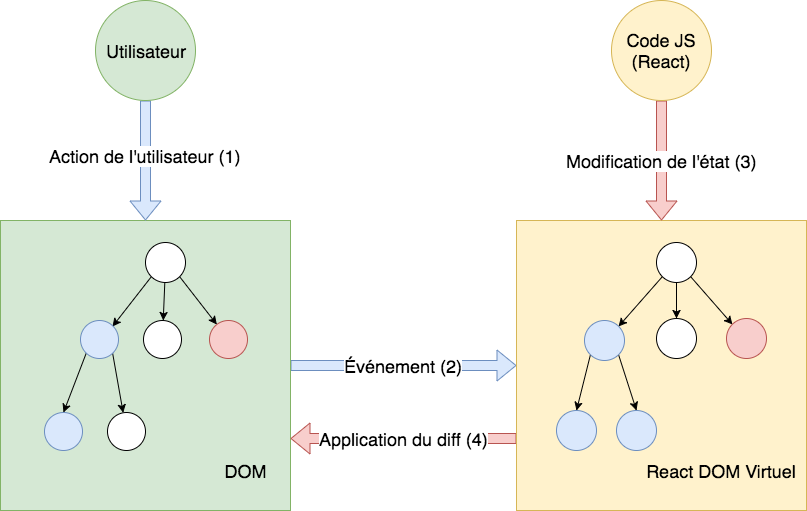
\includegraphics[scale=0.25]{images/schema-react.png}
  \caption{Schéma explicatif du principe de réconciliation de la librairie \texttt{React}}
\end{figure}
\end{frame}

\begin{frame}{\textit{Front-end}}{Outils d'implémentation}
  \begin{block}{JSX}
    \texttt{JSX} est une extension JavaScript dont l'usage est très recommandé lors du développement d'une application \texttt{React}.
  \end{block}
  \begin{figure}[!ht]
    \centering
    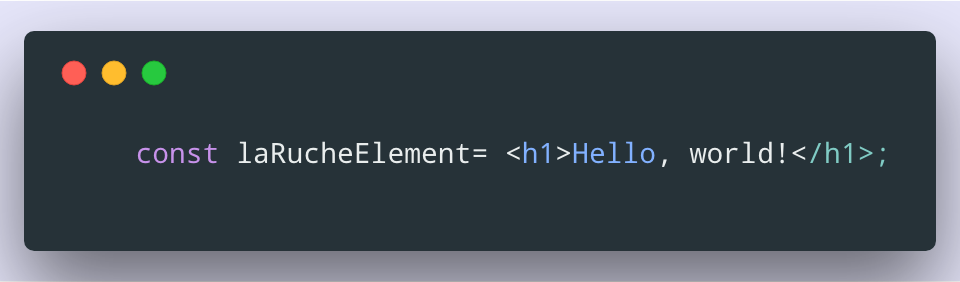
\includegraphics[scale=0.25]{images/JSX3.png}
  \end{figure}
\end{frame}

\subsection{\protect\textit{Back-end}}
\begin{frame}{\textit{Back-end}}{Outils d'implémentation}
%%PHP, MySQL
  \begin{figure}[!htb]
  \minipage{0.25\textwidth}
    
\includegraphics[width=\linewidth, scale=0.03]{images/mysql.png}
  \endminipage\hfill
  \minipage{0.25\textwidth}
    
\includegraphics[width=\linewidth, scale=0.04]{images/php.png}
  \endminipage\hfill
  \minipage{0.25\textwidth}
    
\includegraphics[width=\linewidth, scale=0.15]{images/symfony.png}
  \endminipage
  \end{figure}

  \begin{description}
    \item[Langage de développement :] Serveur codé en PHP et le framework \texttt{Symfony} pour un système modulaire basé sur le \textit{design pattern} \textbf{MVC}.
    \item[Base de données :] Base de données relationnelle mise en place via MySQL interagissant avec l'\textbf{ORM} \texttt{Doctrine}.
  \end{description}
\end{frame}
%----------------------------------------------------------------------------------------
%   CONCLUSION
%----------------------------------------------------------------------------------------
\section{Conclusion}
\subsection{Écosystème décentralisé/autonome et extensible}
\begin{frame}{Écosystème décentralisé/autonome et extensible}{Conclusion}

\begin{block}{Décenstralisation/Autonomie}
\begin{enumerate}
  \item Réseau de ruches \textbf{décenstralisé} : ensemble de ruches indépendantes et coopératives ne répondant à aucune entité centrale.
  \item Les fournisseurs sont \textbf{autonomes} : responsables de la formation des ruches et de l'organisation des évènements de collecte.
\end{enumerate}
\end{block}

\begin{block}{Extensibilité}
Le système est \textbf{versatile} et \textbf{extensible} : extension des ruches, augmentation de leur nombre, ajout de fonctionnalités supplémentaires, $\dots$.
\end{block}
\end{frame}

\subsection{Perspectives}
\begin{frame}{Perspectives}{Conclusion}
 \begin{itemize}
   \item Changement du nom du projet
   \item Récolte de \textit{feedback} des utilisateurs potentiels
   \item Optimisation de la logistique
   \item Implémentation de fonctionnalités supplémentaires (paiement en ligne, commandes retardées, portefeuille virtuel, $\dots$)
   \item Internationalisation
 \end{itemize}
\end{frame}
\end{document}
